\documentclass[a4paper,10pt]{book}
\usepackage[utf8]{inputenc}
\usepackage{graphicx}
\usepackage{amsmath}
\usepackage{url}

%opening
\title{}
\author{}

\begin{document}
\chapter{18 de setembro}

\section{Definição}

A transformada de Laplace é definida como:
$$F(s)=\mathcal{L}\{ f(t)\} := \int_0^\infty f(t)e^{-st}dt,~~\Re(s)>s_0$$

 Exemplo:
 
 $$f(t)=1$$
 \begin{eqnarray*}
  F(s) &=& \int_0^\infty f(t)e^{-st}dt\\
  &=&\int_0^\infty e^{-st}dt\\
  &=&\left.\frac{e^{-st}}{-s}\right|_{t=0}^{t \to \infty}\\
  &=& \frac{0-1}{-s}=\frac{1}{s}, ~~s>0.
 \end{eqnarray*}
% 

Exemplo:
 $$f(t)=e^{as}$$
 
 
 \begin{eqnarray*}
  F(s) &=& \int_0^\infty f(t)e^{-st}dt\\
  &=&\int_0^\infty e^{at}e^{-st}dt\\
    &=&\int_0^\infty e^{(a-s)t}dt\\
    &=&\left.\frac{e^{(a-s)t}}{a-s}\right|_0^\infty\\
    &=&\frac{0-1}{a-s}\\
    &=&\frac{1}{s-a},~~~s>a.
 \end{eqnarray*}
% 
% 
% 
 \section{Propriedade da linearidade}
% 
 $$\mathcal{L}\{\alpha f(t)+\beta g(t)\}=\alpha\mathcal{L}\{ f(t)\}+\beta\mathcal{L}\{ g(t)\}$$

 exemplo:
 
 \begin{eqnarray*}
\mathcal{L}\{3+2 e^{t}\}&=&3\mathcal{L}\{ 1\}+2\mathcal{L}\{ e^t\} \\
&=&\frac{3}{s}+\frac{2}{s-1}
 \end{eqnarray*}

 % 
% 
 \section{Propriedade da derivada}
 $$\mathcal{L}\{f'(t)\}=s\mathcal{L}\{ f(t)\}-f(0)$$

 Exemplo:
 
 $$f(t)=t$$
 $$f'(t)=1$$
 
 $$\mathcal{L}\{1\}=s\mathcal{L}\{ t\}-0$$
 $$\mathcal{L}\{ t\} = \frac{1}{s^2}$$


  Exemplo:
 
 $$f(t)=t^2$$
 $$f'(t)=2t$$
 
 $$\mathcal{L}\{2t\}=s\mathcal{L}\{ t^2\}-0$$
 $$\mathcal{L}\{ t^2\} = \frac{2}{s^3}$$

 
 Analogamente:
 $$\mathcal{L}\{ t^3\} = \frac{6}{s^4}$$

  $$\mathcal{L}\{ t^n\} = \frac{n!}{s^{n+1}}$$
  
  
  
  Aplicação:
  
  $$f'(t)+f(t) = 1$$
  com $f(0)=1$.

  Aplicando a transformada de Laplace, temos:
  
  $$\left[sF(s)-f(0)\right]+F(s)=\frac{1}{s}$$
  
  $$F(s)(s+1) = \frac{1}{s}+1$$
  
  $$F(s) = \frac{1}{s(s+1)}+\frac{1}{(s+1)}$$
  
  $$F(s) = \frac{1+s}{s(s+1)}=\frac{1}{s}$$
  
  $$f(t)=1$$
  
  OBS: $f(t)=1, t\neq 2$,  $f(2)=0$.
  
  
  \chapter{21 de setembro}

  \section{A transformada inversa}
  
  Se $\mathcal{L}\{f(t)\}=F(s)$, dizemos que $f(t)$ é a transformada inversa de $F(s)$:
  $$\mathcal{L}^ {-1}(F(s))=f(t)$$
  
  \section{Propriedade da derivada - derivada segunda}
 Vimos a propriedade da derivada:
    $$\mathcal{L}\{f'(t)\}=s\mathcal{L}\{ f(t)\}-f(0)$$
 
 Agora aplicamos à derivada da função $f'(t)$:
 \begin{eqnarray*}
 \mathcal{L}\{f''(t)\}&=&s\mathcal{L}\{ f'(t)\}-f'(0)\\
 &=&s\left[sF(s)-f(0)\right]-f'(0)\\
 &=&s^2F(s)-sf(0)-f'(0)\\
 \end{eqnarray*}

 Analogamente:
 \begin{eqnarray*}
 \mathcal{L}\{f'''(t)\}
  &=&s^3F(s)-s^2f(0)-sf'(0)-f''(0)\\
 \end{eqnarray*}

 
 % 
 Exemplo:
 \begin{eqnarray*}f(t)&=&\cos(\omega t)\\
 f'(t)&=&-\omega\sin(\omega t)\\
 f''(t)&=&-\omega^2\cos(\omega t)
 \end{eqnarray*}
 
 isto é:
 $$f''(t)=-\omega^2f(t)$$
 Aplicando a transformada de Laplace, temos:
 \begin{eqnarray*}
 \mathcal{L}\{f''(t)\}&=&-\omega^2\mathcal{L}\{ f(t)\}.
 \end{eqnarray*}
 Usamos a propriedade da derivada (segunda):
 \begin{eqnarray*}
 s^2F(s)-sf(0)-f'(0)&=&-\omega^2F(s)
 \end{eqnarray*}
 isto é:
 \begin{eqnarray*}
 (s^2+\omega^2)F(s)=sf(0)+f'(0)=s
 \end{eqnarray*}
 Portanto:
 $$F(s)=\mathcal{L}\{\cos(\omega t)\}=\frac{s}{s^2+\omega^2},~~s>0$$
% 
 Analogamente, temos:
 $$\mathcal{L}\{\sin(\omega t)\}=\frac{w}{s^2+\omega^2}$$
 
 \section{Método das frações parciais para calcular transformadas inversas
 }
% * Ler seção 3.4 do livro. %https://www.ufrgs.br/reamat/TransformadasIntegrais/livro-tl/apdleatdd-mx00e9todo_das_frax00e7x00f5es_parciais_para_calcular_transformadasinversas.html
% 
 \begin{eqnarray*}F(s)&=&\frac{s^2-6s+4}{s^3-3s^2+2s}\\
 &=&\frac{s^2-6s+4}{s(s^2-3s+2)}\\
 &=&\frac{s^2-6s+4}{s(s-1)(s-2)}\\
 &=&\frac{A}{s}+\frac{B}{s-1}+\frac{C}{s-2}
 \end{eqnarray*}
% 
 O teorema das frações parciais garante que existem constantes $A$, $B$ e $C$ tais que:
 \begin{eqnarray}\label{eq_or_fp}\frac{s^2-6s+4}{s(s-1)(s-2)}
 &=&\frac{A}{s}+\frac{B}{s-1}+\frac{C}{s-2}
 \end{eqnarray}
 para todo $s$ complexo.

 
Primeiro multiplicamos (\ref{eq_or_fp}) por $s$:
\begin{eqnarray*}\frac{s^2-6s+4}{(s-1)(s-2)}
 &=&A+\frac{Bs}{s-1}+\frac{Cs}{s-2}
 \end{eqnarray*}
Substituindo $s$ por $0$, temos:
\begin{eqnarray*}\frac{4}{(-1)(-2)}
 =A~~~\Longrightarrow ~~ A=2
 \end{eqnarray*}

 
Agora multiplicamos a expressão (\ref{eq_or_fp}) por $s-1$:
% 
 \begin{eqnarray*}\frac{s^2-6s+4}{s(s-2)}
 &=&\frac{A(s-1)}{s}+{B}+\frac{C(s-1)}{s-2}
 \end{eqnarray*}

 Substituindo $s$ por 1, temos:

  \begin{eqnarray*}\frac{1-6+4}{1(1-2)}
 =B~~~\Longrightarrow ~~B = 1
 \end{eqnarray*}

 Finalmente multiplicamos (\ref{eq_or_fp}) por $s-2$:
 % 
 
 \begin{eqnarray*}\frac{s^2-6s+4}{s(s-1)}
 &=&\frac{A(s-2)}{s}+\frac{B(s-2)}{s-1}+{C}
 \end{eqnarray*}
E substuimos por $s=2$:

 \begin{eqnarray*}\frac{4-12+4}{2(2-1)}
 ={C}~~~\Longrightarrow ~~C = -2
 \end{eqnarray*}

 
 \begin{eqnarray}F(s)&=&\frac{s^2-6s+4}{s(s-1)(s-2)}\\
 &=&\frac{2}{s}+\frac{1}{s-1}-\frac{2}{s-2}
 \end{eqnarray}
 
 Olhanda na tabela, encontramos:
 $$f(t)=2+e^t-2e^{2t},~~t\geq 0$$
 Tabela com item 1 e item 7 com $a=1$ e $a=2$.
 
 {\bf Obs:}
 
 $$F(s)=\frac{s}{(s^2+1)(s-2)^3}=\frac{A+Bs}{s^2+1}+\frac{C}{(s-2)}+\frac{D}{(s-2)^2}+\frac{E}{(s-2)^3}$$
 % 
  \section{Propriedade de translação no eixo s}
% 
  Se $F(s)$ é a transformada de Laplace de $f(t)$ definida para $s>s_0$, então $e^{at}f(t)$ é a transformada inversa de $F(s-a)$, isto é
  \begin{equation*}
  \mathcal{L}\left\{e^{at}f(t)\right\} =F(s-a),\qquad s>s_0+a
  \end{equation*}
  A demostração vem da aplicação da definição da transformada de Laplace $F(s-a)$:
 \begin{eqnarray*}
   F(s-a)&=&\int_0^\infty f(t)e^{-(s-a)t}dt\\
  &=&\int_0^\infty f(t)e^{at}e^{-st}dt\\
&=&\int_0^\infty \left(f(t)e^{at}\right)e^{-st}dt\\
    &=&\mathcal{L}\left\{e^{at}f(t)\right\}
   \end{eqnarray*}

{\bf Exemplo:}
$$\mathcal{L}\left\{t^2\right\}=\frac{2}{s^3}$$
   
$$\mathcal{L}\left\{t^2e^{at}\right\}=\frac{2}{(s-a)^3}$$
   
   %  
  \section{Oscilador harmônico}
%  %https://www.ufrgs.br/reamat/TransformadasIntegrais/livro-tl/apdtedtd-aplicax00e7x00e3o_oscilador_harmx00f4nico.html
$$F(s)=\frac{1}{ms^2+\gamma s+ \kappa}$$


Caso $m=1$, $\gamma=0$, $\kappa =4$:

$$F(s)=\frac{1}{s^2+ 4}=\frac{1}{s^2+ 2^2}$$

$$f(t)=\frac{1}{2}\sin(2t)$$

Caso $m=1$, $\gamma=2$, $\kappa =5$:

\begin{eqnarray*}F(s)&=&\frac{1}{s^2+2 s+ 5}\\
&=&\frac{1}{\underbrace{(s+1)^2}_{s^2+2s+1}+4}\\
&=&\frac{1}{(s+1)^2+2^2}\\
&=&G(s+1)
 \end{eqnarray*}
onde $G(s)=\frac{1}{s^2+2^2}$
 
 Como $$g(t)=\mathcal{L}^{-1}\{G(s)\}=\frac{1}{2}\sin(2t)$$ $$f(t)=\frac{1}{2}e^{-t}\sin(2t)$$
Onde usamos o produto notável: $$(s+a)^2=s^2+2as+a^2.$$
 
 Caso $m=1$, $\gamma=3$, $\kappa=2$:
\begin{eqnarray*}F(s)&=&\frac{1}{s^2+3 s+ 2}\\
F(s)&=&\frac{1}{(s+1)(s+2)}\\
 \end{eqnarray*}

 Usando a tabela, encontramos:
 $$f(t)=e^{-t}-e^{-2t}$$
 
 Pergunta: Quantas vezes $f(t)$ para por zero para $t\geq 0$.
 $$f(t)=e^{-t}-e^{-2t}=0$$
 $$e^{-t}(1-e^{-t})=0$$
  Assim $f(t)=0$ se e somente se $e^{-t}=1$, i.e., $t=0$.
  
  
  \chapter{23 de setembro}
  \section{Exemplo de cálculo de transformada de Laplace usando função de Heaviside}
  
 Representar algebricamente em termos da função de Heaviside a função dada no gráfico da figura \ref{fig_Heaviside_4}.
\begin{figure}[!ht]
\begin{center}

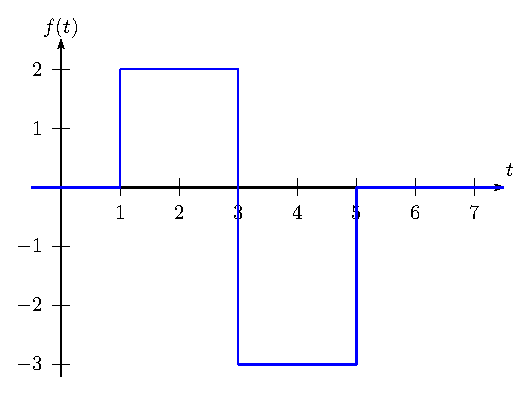
\includegraphics{figs/figura_8}\end{center}
\caption{\label{fig_Heaviside_4}}
\end{figure} 
 Observe que podemos representar $f(t)$ da seguinte forma:
 \begin{equation}
  f(t)=\left\{ \begin{array}{ll} 0, &t<1\\2,&1<t<3\\-3,& 3<t<5\\0,&t>5. \end{array}\right.
 \end{equation}
 Para representar em termos da função de Heaviside, olhe para o gráfico pensando em dois pulsos: $2(u(t-1)-u(t-3))$ e $-3(u(t-3)-u(t-5))$. A soma deles é a função desejada:
 \begin{equation}
 f(t)=2(u(t-1)-u(t-3))-3(u(t-3)-u(t-5)).
 \end{equation}

 \begin{equation}
 f(t)=2u(t-1)-5u(t-3)+3u(t-5).
 \end{equation}
 \begin{figure}[!ht]
\begin{center}

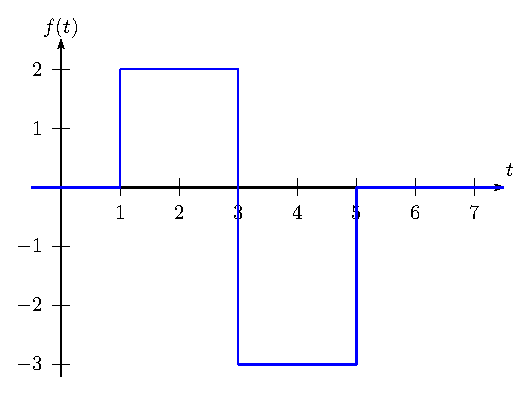
\includegraphics{figs/figura_8}\end{center}
\caption{\label{fig_Heaviside_4}}
\end{figure} 
 $$F(s)=\frac{2e^{s}-5e^{-3s}+3e^{-5s}}{s}$$
onde usamos que
$$\mathcal{L}\{u(t-a)\}=\frac{e^{-as}}{s}$$
O que vamos provar agora.  
 \section{Transformada de Laplace da Heaviside}
% 
 $$f(t)=u(t-a), ~~a>0$$
% 
 \begin{eqnarray*}
  F(s)&=&\int_0^\infty f(t)e^{-st}dt\\
  &=&\int_0^\infty u(t-a)e^{-st}dt\\
&=&\int_0^a \underbrace{u(t-a)}_{0}e^{-st}dt + \int_a^\infty \underbrace{u(t-a)}_{1}e^{-st}dt\\
&=& \int_a^\infty e^{-st}dt\\
&=&\left.\frac{e^{-st}}{-s}\right|_{t=a}^\infty\\
&=&\frac{e^{-as}}{s},~~s>0
\end{eqnarray*}
% 
 \section{Propriedade do deslocamento no tempo}
% 
   Se $F(s)$ é a transformada de $f(t)$, então $f(t-a)u(t-a)$ é a transformada inversa de $e^{-as}F(s)$, isto é
 \begin{equation}
 \mathcal{L}\left\{u(t-a)f(t-a)\right\} =e^{-as}F(s),\qquad a>0
 \end{equation}
 ou
 \begin{equation}{\label{eq_trans_t_inv}}
 \mathcal{L}^{-1} \left\{e^{-as}F(s)\right\} =u(t-a)f(t-a),\qquad a>0.
 \end{equation} 
%  
 Dem: Aplicamos a definição da transformada de Laplace e obtemos:
  \begin{eqnarray*}
  \mathcal{L}\left\{u(t-a)f(t-a)\right\}&=&\int_0^\infty u(t-a)f(t-a)e^{-st}dt\\
  &=&\int_0^a \underbrace{u(t-a)}_{0}f(t-a)e^{-st}dt+\int_a^\infty \underbrace{u(t-a)}_{1}f(t-a)e^{-st}dt\\
  &=&\int_a^\infty f(t-a)e^{-st}dt,
  \end{eqnarray*}
  pois $u(t-a)$ é zero no intervalo $[0,a)$ e um no intervalo $(a,\infty)$. Depois usamos a mudança de variável $v=t-a$ na última integral:
  \begin{equation*}
  \int_a^\infty f(t-a)e^{-st}dt=\int_0^\infty f(v)e^{-s(v+a)}dv=e^{-as}\int_0^\infty f(v)e^{-sv}dv.
  \end{equation*}
  Logo,
  \begin{equation}
  \mathcal{L}\left\{u(t-a)f(t-a)\right\}=e^{-as}\mathcal{L}\left\{f(t)\right\}=e^{-as}F(s).
  \end{equation}
% 
  Observe que tomando $f(t)=1$ na propriedade do deslocamento, temos:
  \begin{equation}{\label{Heaviside_trans_1}}
  \mathcal{L}\left\{1~\!u(t-a)\right\} =\frac{e^{-as}}{s},\qquad a>0
  \end{equation}
  que coincide com a fórmula da transformada de Laplace da Heaviside. %
  Quando $a=0$ na equação acima, recaímos no item 1 da tabela de transformadas.
 
  

{\bf Exemplo} Aplicando diretamente a propriedade do deslocamento em $t$ e usando que $\mathcal{L}\{t^2\}=\frac{2}{s^3}$, calculamos a transformada inversa de Laplace de $e^{-3s}\frac{2}{s^3}$:
  \begin{equation}
  \mathcal{L}^{-1}\left\{e^{-3s}\frac{2}{s^3}\right\}=u(t-3)(t-3)^2.
  \end{equation}
Cuidado:
  \begin{equation}
  u(t-3)(t-3)^2 \neq u(t-3)t^2.
  \end{equation}

  %  
%  
%   
   {\bf Exemplo:}
   Vamos calcular a transformada inversa de Laplace da função
  \begin{equation}
  F(s)=e^{-s}\frac{1}{(s+1)^2-1}.
  \end{equation}
{\bf Obs:} As raizes do denominador são:
$$(s+1)^2-1=0$$
  $$(s+1)^2=1$$
  $$(s+1) = \pm 1$$
  $$s = -1\pm 1$$
  
    Primeiro calculamos a transformada de $\frac{1}{(s+1)^2-1}$ usando a propriedade.
   \begin{eqnarray*}
   \mathcal{L}^{-1}\left\{\frac{1}{(s+1)^2-1}\right\}&=&e^{-t}\sinh(t)\\
   &=&e^{-t}\left(\frac{e^{t}-e^{-t}}{2}\right)\\
   &=&\frac{1-2e^{-2t}}{2}
 \end{eqnarray*}
  Depois usamos a propriedade  para concluir
  \begin{equation}
  \mathcal{L}^{-1}\left\{e^{-s}\frac{1}{(s+1)^2-1}\right\}=u(t-1)\mathcal{L}^{-1}\left\{\frac{1}{(s+1)^2-1}\right\}
  _{t\to t-1}=u(t-1)e^{-(t-1)}\sinh(t-1).
   \end{equation}
% % 
%   
%   
%   
 \section{A propriedade da transformada de Laplace da integral de uma função}
  Se $F(s)$ é a transformada de Laplace de uma função contínua por partes $f(t)$, então $\int_0^tf(\tau)d\tau$ é a transformada inversa de $\frac{1}{s}F(s)$, isto é
 \begin{equation}{\label{eq_trans_int}}
 \mathcal{L}\left\{\int_0^tf(\tau)d\tau\right\} =\frac{1}{s}F(s),
 \end{equation}
 ou
 \begin{equation}{\label{eq_trans_int_inv}}
 \mathcal{L}^{-1} \left\{\frac{1}{s}F(s)\right\} =\int_0^tf(\tau)d\tau.
 \end{equation} 
% 
Dem: Seja $g(t)=\int_0^tf(\tau)d\tau$. Então $g'(t)=f(t)$. Aplicamos a propriedade da transformada da derivada  e temos:
 \begin{equation}
 \mathcal{L}\{g'(t)\}=s\mathcal{L}\{g(t)\}-g(0).
 \end{equation}
 Usando o fato que $g(0)=0$, temos
 \begin{eqnarray*}
 \mathcal{L}\left\{\int_0^tf(\tau)d\tau\right\}&=&\mathcal{L}\left\{g(t)\right\}\\
 &=&\frac{1}{s}\mathcal{L}\{g'(t)\}\\
 &=&\frac{1}{s}\mathcal{L}\{f(t)\}\\
 &=&\frac{1}{s}F(s).
 \end{eqnarray*}
% 
% 
  
  \chapter{Dia 25 de setembro}
  \section{Oscilador harmônico - regime de amortecimento}
  
  Ver aula no 
  \url{https://colab.research.google.com/drive/197QbUeLlV2GEulEhjyVfpBeNRngxLls3}
  
  \noindent Mais exemplos de PVI em:
  \url{https://colab.research.google.com/drive/1MTC1GSOP_DLPYZusqohP9DcaWr_ab-UX}
  
  
   \section{Delta de dirac}
   Muitos fenômenos físicos exigem a representação de uma força muito grande em um intervalo de tempo muito pequeno, por exemplo:
 \begin{itemize}
  \item um circuito elétrico recebe uma força eletromotriz grande em um curto intervalo de tempo.
  \item um sistema massa-mola é atingido por uma martelo.
  \item uma bola de futebol parada recebe um chute, ou seja, uma força quase instantânea, que a coloca em movimento.
  \item um avião é atingido por um raio.
 \end{itemize}
 Para representar essa força, vamos tomar a função pulso unitário em um curto intervalo de tempo $[-\epsilon,\epsilon]$ em torno da origem, isto é, um pulso com integral unitária:
 \begin{equation}
 \delta_\epsilon(t)=\frac{1}{2\epsilon}\left(u(t+\epsilon)-u(t-\epsilon)\right)=\left\{\begin{array}{ll}0,&t<-\epsilon\\ \frac{1}{2\epsilon},&-\epsilon<t<\epsilon\\0,&t>\epsilon.\end{array}\right.
 \end{equation}
 Um pulso unitário em torno de $t=a$ é representado por
 \begin{equation}{\label{def_delta_dirac}}
 \delta_\epsilon(t-a)=\frac{1}{2\epsilon}\left(u(t-(a-\epsilon))-u(t-(a+\epsilon))\right)=\left\{\begin{array}{ll}0,&t<a-\epsilon\\ \frac{1}{2\epsilon},&a-\epsilon<t<a+\epsilon\\0,&t>a+\epsilon.\end{array}\right.
 \end{equation}
 Observe que $\int_{-\infty}^\infty\delta_\epsilon(t-a)=1$ para qualquer $\epsilon>0$. A figura \ref{fig_delta_dirac} apresenta o gráfico de $\delta_\epsilon(t-a)$ para $a>0$ e $\epsilon=1$, $\epsilon=\frac{1}{2}$, $\epsilon=\frac{1}{4}$, $\epsilon=\frac{1}{8}$ e $\epsilon=\frac{1}{12}$.
 A função que representa uma grande força instantânea é chamada de {\bf função impulso} ou {\bf função Delta de Dirac} e pode ser definida pelo limite das funções pulsos:
 \begin{equation}
 \delta(t-a)=\lim_{\epsilon\to 0}\delta_\epsilon(t-a).
 \end{equation}
 Este limite não pode ser interpretado pontualmente, isto é, como o limite usual de funções reais, mas apenas no contexto de uma integral, como veremos.
 A figura \ref{fig_delta_dirac} apresenta o gráfico de $\delta_\epsilon(t-a)$ quando $\epsilon$ diminui e uma representação gráfica para $\delta(t-a)$.
% 
%   
 \begin{figure}[!ht]
 \begin{center}
% 
 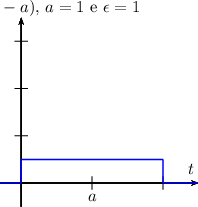
\includegraphics{figs/figura_1}\hspace{20pt}
 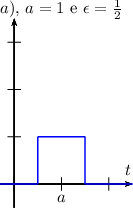
\includegraphics{figs/figura_2}\hspace{20pt}
 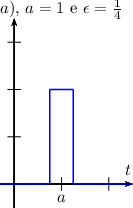
\includegraphics{figs/figura_3}
 
 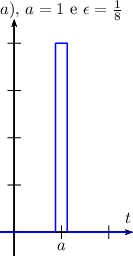
\includegraphics{figs/figura_4}\hspace{20pt}
 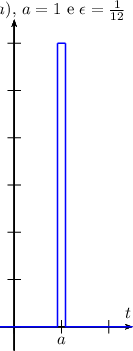
\includegraphics{figs/figura_5}\hspace{20pt}
 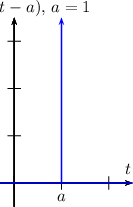
\includegraphics{figs/figura_6}
 \end{center}
 \caption{\label{fig_delta_dirac}}
 \end{figure}
% 
 {\bf Obs:}A função delta de Dirac pode ser definida como limite de outras sequências de funções com propriedades análogas a sequência de pulsos. Por exemplo, podemos definir $\delta(t)$ como limite das funções
 \begin{equation}
 f_\epsilon(t)=\frac{1}{\epsilon\sqrt{\pi}}e^{-\frac{t^2}{\epsilon^2}}
 \end{equation}
% 
% 
% 
 A função Impulso é zero em todo ponto, exceto em $t=a$:
 \begin{equation}
 \delta(t-a)=\left\{\begin{array}{ll}0,&t\neq a\\\infty,&t=a  \end{array}\right.
 \end{equation}
 e
 \begin{equation}
 \int_{-\infty}^\infty\delta(t-a)dt=1
 \end{equation}
 A função Delta de Dirac deve ser sempre compreendida como o limite de funções reais no contexto de uma integração, isto conduz à chamada  {\bf propriedade da filtragem}, que define totalmente a Delta da Dirac:
 Se $f(t)$ for um função contínua em torno de $t=a$, então
 \begin{equation}{\label{prop_filtragem_dirac}}
 \int_{-\infty}^\infty \delta(t-a)f(t)dt=f(a). 
 \end{equation}
 Para chegar a esta conclusão, definimos $F(t)=\int_a^t f(\tau)d\tau$ e calculamos:
 \begin{eqnarray*}
 \int_{-\infty}^\infty \delta(t-a)f(t)dt&=&\lim_{\varepsilon\to 0+}
 \int_{-\infty}^\infty \delta_\varepsilon(t-a)f(t)dt\\
 &=&\lim_{\varepsilon\to 0+}\frac{1}{2\varepsilon}\int_{-a+\varepsilon}^{a+\varepsilon} f(t)dt\\
 &=&\lim_{\varepsilon\to 0+}\frac{F(\varepsilon)-F(-\varepsilon)}{2\varepsilon}\\
 &=&F'(0)=f(a).
 \end{eqnarray*}
 \subsection{Delta de Dirac como derivada distribucional da função Heaviside}
 Na equação (\ref{def_delta_dirac}) definimos a função Delta de Dirac como
 \begin{equation}
 \delta(t-a)=\lim_{\epsilon\to 0}\frac{1}{2\epsilon}\left(u(t-(a-\epsilon))-u(t-(a+\epsilon))\right).
 \end{equation}
 Por outro lado, usamos a definição de derivada para escrever
 \begin{equation}
 \lim_{\epsilon\to 0}\frac{1}{2\epsilon}\left(u((t-a)+\epsilon))-u((t-a)-\epsilon))\right)=\frac{d}{dt}u(t-a)
 \end{equation}
 ou seja,
 \begin{equation}
 \delta(t-a)=\frac{d}{dt}u(t-a).
 \end{equation}
 Observe que as funções de Heaviside e de Dirac não são funções no sentido do cálculo diferencial e integral. Naturalmente, a derivada acima também vale somente num sentido generalizado, mas é coerente quando olhamos a função de Heaviside como limite de funções rampas (ver figura \ref{fig_Heaviside_1}), pois na origem a derivada tende ao infinito.
% A transformada de Laplace de função Delta de Dirac é obtido pela propriedade da filtragem dada na equação (\ref{prop_filtragem_dirac}):
% \begin{equation}{\label{prop_trans_delta_dirac}}
% \mathcal{L}\{\delta(t-a)\}=\int_0^\infty \delta(t-a)e^{-st}dt=e^{-as}.
% \end{equation}
% 
% 
% \section{Circuto RLC}
% 
% 
% \section{Aplicação: circuito RLC}{\label{sec_circ_2}}
% Ver \url{https://colab.research.google.com/drive/1R3rCOc8zv70rSwCf7W30yQlleP6J2Mf2}
% 
% Considere o circuito Resistor/Capacitor/Indutor representado na figura \ref{fig_circ_2} com uma tensão $V(t)$ aplicada do tipo pulso,
% \begin{equation}
% V(t)=V_0\left(u(t-a)-u(t-b)\right).
% \end{equation}
% \begin{figure}[!ht]
% \begin{center}
% 
% 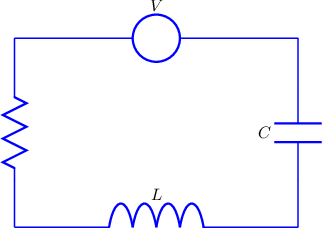
\includegraphics{figs/figura_7_RLC}\end{center}
% \caption{\label{fig_circ_2}}
% \end{figure} 
% O modelo para a corrente $i(t)$ obedece a lei de Kirchoff:
% \begin{equation}{\label{modelo_corrente}}
% Li'(t)+ Ri(t)+\frac{1}{C}q(t)=V_0\left(u(t-a)-u(t-b)\right),
% \end{equation}
% onde $q(t)$ é a carga no capacitor, $\frac{1}{C}q(t)$ é a tensão no capacitor de capacitância $C$, $Ri(t)$ é a tensão no resistor de resistência $R$ e $Li'(t)$ é a tensão no indutor de indutância $L$. Considere as condições iniciais $i(0)=0$ e $q(0)=0$.
% Dado que $\frac{dq(t)}{dt}=i(t)$, derivamos a equação do circutio para obter a seguinte equação diferencial:
% \begin{equation}{\label{modelo_corrente_2}}
% Li''(t)+ Ri'(t)+\frac{1}{C}i(t)=V_0\left(\delta(t-a)-\delta(t-b)\right),
% \end{equation}
% onde usamos que a derivada da função de Heaviside é a função delta de Dirac. As condições iniciais para a equação (\ref{modelo_corrente_2}) são $i'(0)=0$ e $i(0)=0$. Com o objetivo de resolver a problema de valor inicial, aplicamos a transformada de Laplace para obter a equação subsidiária
% \begin{equation*}
% Ls^2I(s)+ RsI(s)+\frac{1}{C}I(s)=V_0\left(e^{-as}-e^{-bs}\right),
% \end{equation*}
% que tem solução
% 
% 
% \begin{eqnarray*}
% I(s)&=&\frac{V_0\left(e^{-as}-e^{-bs}\right)}{Ls^2+Rs+\frac{1}{C}}\\
% &=&\frac{1}{L}\frac{V_0\left(e^{-as}-e^{-bs}\right)}{\left(s+\frac{R}{2L}\right)^2-\left(\frac{R}{2L}\right)^2+\frac{1}{LC}}\\
% &=&\frac{V_0}{L}\left[\frac{e^{-as}}{\left(s+\frac{R}{2L}\right)^2+\eta}-\frac{e^{-bs}}{\left(s+\frac{R}{2L}\right)^2+\eta}\right]
% \end{eqnarray*}
% onde
% \begin{equation}
% \eta=\frac{1}{LC}-\left(\frac{R}{2L}\right)^2.
% \end{equation}
% Vamos exemplificar os casos subamortecido, superamortecido e criticamente amortecido tomando $V_0=10V$, $a=1$ e $b=5$:
% \begin{itemize}
%  \item Caso subamortecido ($\eta>0$): escolhemos o caso onde $L=1\ \!$H, $C=\frac{1}{10}\ \!$F e $R=2\Omega$. Nesse caso
%  \begin{equation}
%  I(s)=10\left[\frac{e^{-s}}{\left(s+1\right)^2+9}-\frac{e^{-5s}}{\left(s+1\right)^2+9}\right].
%  \end{equation}
%  Logo,
%  \begin{equation}
%  i(t)=\frac{10}{3}\left(u(t-1)e^{-(t-1)}\sin\left(3 (t-1)\right)-u(t-5) e^{-(t-5)}\sin\left(3 (t-5)\right)\right).
%  \end{equation}
%  O gráfico da corrente é apresentado na figura \ref{fig_circ_RCL_1}.
% \begin{figure}[!ht]
% \begin{center}
% 
% 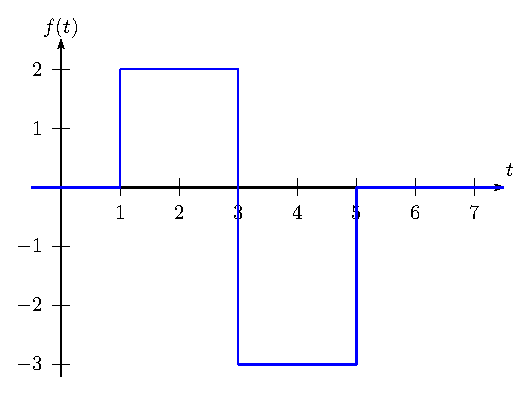
\includegraphics{figs/figura_8}\end{center}
% \caption{\label{fig_circ_RCL_1}}
% \end{figure}
%  \item Caso superamortecido ($\eta<0$): escolhemos o caso onde $L=1\ \!$H, $C=1\ \!$F e $R=4\Omega$. Nesse caso
%  \begin{equation}
%  I(s)=10\left[\frac{e^{-s}}{\left(s+2\right)^2-3 }-\frac{e^{-5s}}{\left(s+2\right)^2-3}\right].
%  \end{equation}
%  Logo,
%  \begin{eqnarray*}
%  i(t)&=&10\left(u(t-1)\frac{e^{-2(t-1)}}{ \sqrt{3}}\sinh\left(\sqrt{3} (t-1)\right)-u(t-5)\frac{e^{-2(t-5)}}{\sqrt{3} }\sinh\left(\sqrt{3}  (t-5)\right)\right)\\
%  &=&\frac{5}{\sqrt{3}}u(t-1)\left(e^{\left(\sqrt{3}-2\right) (t-1)}-e^{-\left(\sqrt{3}+2\right) (t-1)}\right)+\\
%  &+&\frac{5}{\sqrt{3}}u(t-5)\left(e^{\left(\sqrt{3}-2\right) (t-5)}-e^{-\left(\sqrt{3}+2\right) (t-5)}\right)
%  \end{eqnarray*}
%  O gráfico da corrente é apresentado na figura \ref{fig_circ_RCL_2}.
% \begin{figure}[!ht]
% \begin{center}
% 
% 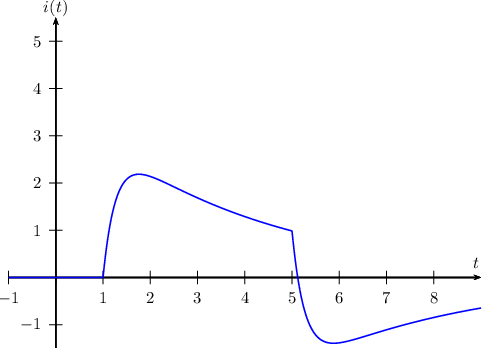
\includegraphics{figs/figura_9}\end{center}
% \caption{\label{fig_circ_RCL_2}}
% \end{figure}
% \item Caso criticamente amortecido ($\eta=0$): escolhemos o caso onde $L=1\ \!$H, $C=1\ \!$F e $R=2\Omega$. Nesse caso
%  \begin{equation}
%  I(s)=10\left[\frac{e^{-s}}{\left(s+1\right)^2}-\frac{e^{-5s}}{\left(s+1\right)^2}\right].
%  \end{equation}
%  Logo,
%  \begin{equation}
%  i(t)=10\left(u(t-1)e^{-(t-1)} (t-1)-u(t-5)e^{-(t-5)} (t-5)\right).
%  \end{equation}
% O gráfico da corrente é apresentado na figura \ref{fig_circ_RCL_3}.
% \begin{figure}[!ht]
% \begin{center}
% 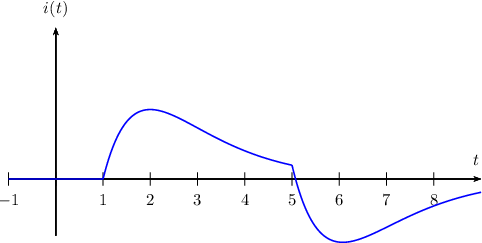
\includegraphics{figs/figura_10}\end{center}
% \caption{\label{fig_circ_RCL_3}}
% \end{figure}
% \end{itemize}
% 
%   
\end{document}
  
